\section{Problemstellung}

%----------------------------------------------------------------------%SLIDE -
\begin{frame}
    \frametitle{Problemstellung}
    Ziel:
    \begin{itemize}
        \item
            Neuronale Netzwerke zu trainieren, so dass diese uns im Go schlagen können.
    \end{itemize}    
    Zwischenziel:
    \begin{itemize}
        \item
            Netze zu trainieren, so dass sie besser als zufällig erzeugte Netze spielen.
    \end{itemize}
\end{frame}
%----------------------------------------------------------------------%SLIDE -

%----------------------------------------------------------------------%SLIDE -
\begin{frame}
    \frametitle{Go}
    \begin{columns}
        \column{0.5\textwidth}
        \begin{itemize}
            \item Asiatisches Brettspiel
            \item Wird auf Brettern mit $19 \times 19$ Knoten gespielt.
            \item Ziel: Gebiet einkreisen und gegnerische Steine schlagen
            \item Spielende: wenn beide Spieler passen
        \end{itemize}
        \column{0.5\textwidth}
        \begin{figure}
            \centering
            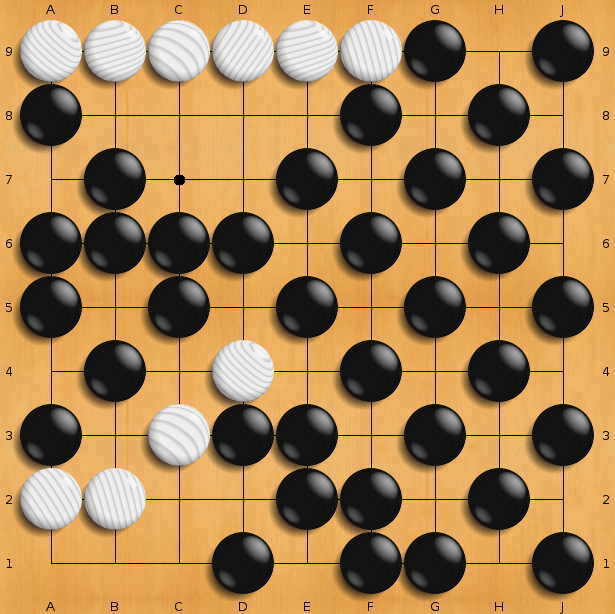
\includegraphics[scale=0.25]{content/img/go_board}
            \caption{generated with qGo}
        \end{figure}
    \end{columns}
\end{frame}
%----------------------------------------------------------------------%SLIDE -

%----------------------------------------------------------------------%SLIDE -
\begin{frame}
    \frametitle{Neuronale Netzwerke}
    \begin{itemize}
        \item Besteht aus mehreren Schichten (Layer)
        \item Layer bestehen aus Neuronen
        \item Neuronen benachbarter Layer sind alle durch Kanten untereinander verbunden
        \item Neuronen berechnen ihre Werte durch Aufsummieren aller eingehenden Kantengewichte multipliziert mit den Werten an den ausgehenden Neuronen
        \item Sigmoid Funktion wird auf das Ergebnis angewandt, sodass alle Werte zwischen 0 und 1 sind.
    \end{itemize}
\end{frame}
%----------------------------------------------------------------------%SLIDE -

%----------------------------------------------------------------------%SLIDE -
\begin{frame}
    \frametitle{Neuronale Netzwerke}
    \begin{figure}
        \centering
        % nnet example
\begin{tikzpicture}
    [
        vertex/.style={circle, scale=1.2, draw,},
        edge/.style={-latex,},
        scale=1.5,
    ]

    \node (I1) at (0,0.5)  [vertex] {};
    \node (I2) at (0,1.5)  [vertex] {};
    \node (IT) at (0,3)    [vertex, scale=0.5] {T};
    \node (B1) at (2,0)    [vertex] {};
    \node (B2) at (2,1)    [vertex] {};
    \node (B3) at (2,2)    [vertex] {};
    \node (BT) at (2,3)    [vertex, scale=0.5] {T};
    \node (C1) at (5,0)    [vertex] {};
    \node (C2) at (5,1)    [vertex] {};
    \node (C3) at (5,2)    [vertex] {};
    \node (CT) at (5,3)    [vertex, scale=0.5] {T};
    \node (O1) at (7,0.5)  [vertex] {};
    \node (O2) at (7,1.5)  [vertex] {};

    \node at (0,4) {Input Layer};
    \node at (3.5,4) {Hidden Layer};
    \node at (7,4) {Output Layer};
    \draw [
        decorate,
        decoration={brace, amplitude=5},
    ] (-0.5,3.5) -- (0.5,3.5);
    \draw [
        decorate,
        decoration={brace, amplitude=5},
    ] (1.5,3.5) -- (5.5,3.5);
    \draw [
        decorate,
        decoration={brace, amplitude=5},
    ] (6.5,3.5) -- (7.5,3.5);

    \draw [edge] (I1) -- (B1);
    \draw [edge] (I1) -- (B2);
    \draw [edge] (I1) -- (B3);
    \draw [edge] (I2) -- (B1);
    \draw [edge] (I2) -- (B2);
    \draw [edge] (I2) -- (B3);
    \draw [edge] (IT) -- (B1);
    \draw [edge] (IT) -- (B2);
    \draw [edge] (IT) -- (B3);

    \draw [
        line width=2,
        line cap=round,
        dash pattern=on 0 off 10,
    ] (3.25,0) -- (3.75,0);
    \draw [
        line width=2,
        line cap=round,
        dash pattern=on 0 off 10,
    ] (3.25,1) -- (3.75,1);
    \draw [
        line width=2,
        line cap=round,
        dash pattern=on 0 off 10,
    ] (3.25,2) -- (3.75,2);
    \draw [
        line width=2,
        line cap=round,
        dash pattern=on 0 off 10,
    ] (3.25,3) -- (3.75,3);

    \draw [dashed] (B1) -- ($ (B1) !.33! (C1) $);
    \draw [edge, dashed] ($ (B1) !.66! (C1) $) -- (C1);
    \draw [dashed] (B1) -- ($ (B1) !.33! (C2) $);
    \draw [edge, dashed] ($ (B1) !.66! (C2) $) -- (C2);
    \draw [dashed] (B1) -- ($ (B1) !.33! (C3) $);
    \draw [edge, dashed] ($ (B1) !.66! (C3) $) -- (C3);

    \draw [dashed] (B2) -- ($ (B2) !.33! (C1) $);
    \draw [edge, dashed] ($ (B2) !.66! (C1) $) -- (C1);
    \draw [dashed] (B2) -- ($ (B2) !.33! (C2) $);
    \draw [edge, dashed] ($ (B2) !.66! (C2) $) -- (C2);
    \draw [dashed] (B2) -- ($ (B2) !.33! (C3) $);
    \draw [edge, dashed] ($ (B2) !.66! (C3) $) -- (C3);

    \draw [dashed] (B3) -- ($ (B3) !.33! (C1) $);
    \draw [edge, dashed] ($ (B3) !.66! (C1) $) -- (C1);
    \draw [dashed] (B3) -- ($ (B3) !.33! (C2) $);
    \draw [edge, dashed] ($ (B3) !.66! (C2) $) -- (C2);
    \draw [dashed] (B3) -- ($ (B3) !.33! (C3) $);
    \draw [edge, dashed] ($ (B3) !.66! (C3) $) -- (C3);

    \draw [dashed] (BT) -- ($ (BT) !.33! (C1) $);
    \draw [edge, dashed] ($ (BT) !.66! (C1) $) -- (C1);
    \draw [dashed] (BT) -- ($ (BT) !.33! (C2) $);
    \draw [edge, dashed] ($ (BT) !.66! (C2) $) -- (C2);
    \draw [dashed] (BT) -- ($ (BT) !.33! (C3) $);
    \draw [edge, dashed] ($ (BT) !.66! (C3) $) -- (C3);

    \draw [edge] (C1) -- (O1);
    \draw [edge] (C1) -- (O2);
    \draw [edge] (C2) -- (O1);
    \draw [edge] (C2) -- (O2);
    \draw [edge] (C3) -- (O1);
    \draw [edge] (C3) -- (O2);
    \draw [edge] (CT) -- (O1);
    \draw [edge] (CT) -- (O2);

\end{tikzpicture}         

        % \caption{Feedforward Netz}
        \label{fig:nnet}
    \end{figure}
\end{frame}
%----------------------------------------------------------------------%SLIDE -
